\documentclass[twocolumn]{article}
\usepackage[english]{babel}
\usepackage[utf8]{inputenc}
\usepackage{amsmath,amssymb,physics,mathtools,blindtext,graphicx}
\usepackage[a4paper,total={7.5in,10in}]{geometry}

\begin{document}
\begin{large}
\section*{Some title}
\subsection*{Introduction}
In quantum mechanics, one is often interested in solving the stationary Schrödinger equation in one dimension:
\begin{equation}
    -\frac{\hbar^2}{2m}u''(x) + V(x)u(x) = Eu.
\end{equation}
This equation can be viewed as an eigenvalue problem $\mathcal{H}u = Eu$ where $\mathcal{H}$ is the hamiltonian given above. The solution $u$ can then be approximated by finding the eigenvalues of the discretized Hamiltonian $H$. In this report, a description will be given on how such an eigenvalue problem can be solved using the inverse power method. The result of applying this method on the following potentials will then be presented. 
\begin{equation*}
    \begin{split}
        &(i) \quad V(x) = \frac{m\omega^2x^2}{2}+\frac{\alpha\hbar\omega}{2}e^{-x^2m\omega/\hbar} - A(\alpha)\\ 
        &(ii) \quad V(x) = \frac{m\omega^3x^2}{2}\left(1+\alpha e^{-x^2m\omega/\hbar}\right) \\ 
    \end{split}
\end{equation*}
The constant $A$ in the first equation $(i)$ makes sure that the lowest point of the potential is zero.  

\subsection*{Discretizing the hamiltonian}
From here on, the Schrödinger equation will be written in the dimensionless form
\begin{equation}
    \label{2apr1953}
    -u''(\xi) + V(\xi)u(\xi) = E'u(\xi)
\end{equation}
and we will only consider square integrable solutions $u$ on the real line and assume that $u(|\xi|\to\infty) = 0$. In order to discretize the hamiltonian, we introduce the gridpoints $\xi_j$ and the approximations of the function $u$ at these gridpoints, $u_j\approx u(\xi_j)$. The step size $h=\xi_{j+1}-\xi_j$ is assumed to be constant. Furthermore, we assume that $\xi_j\in[-L,L]$, where $L$ is chosen such that $u(\xi)\approx 0$ for $|\xi|\geq L$. The second derivative in the hamiltonian can be discretized using finite differences and the second term in the Hamiltonian is discretized in a straightforward manner: $V(\xi_j)u_j$. More details on this is given in an appendix. Using the discretizations, and the fact that $u_j=0$ for large enough $|j|$, the eigenvalue equation $H\mathbf{u} = E\mathbf{u}$ can be set up, where $u_j$ are the elements of $\mathbf{u}$. 
%\begin{equation}
%    H = \frac{1}{12h^2}\left(
%        \begin{matrix}
%            30+12h^2V(\xi_j)  & -16 & 1 & 0 & \dots \\ 
%            -16 & 30 & -16 & 1 & \dots \\ 
%            30 & -16 & 1 & 0 & \dots \\ 
%        \end{matrix}\right)
%\end{equation}

Another approach, which could be used for symmetric potentials, is to assume that the solutions are either even or odd and disregard the negative axis and impose the following boundary conditions:
\begin{equation}
    \begin{rcases}
        &u'(0) = 0 \quad \text{for even } u, \\ 
        &u(0) = 0  \quad \text{for odd } u.
    \end{rcases}
\end{equation} 
%\begin{equation}
%    \begin{split}
%        &u'(0) = 0 \quad\text{and}\quad u(L) = 0 \quad \text{for even } u, \\ 
%        &u(0) = 0 \quad\text{and}\quad u(L) = 0 \quad \text{for odd } u.
%    \end{split}
%\end{equation} 
This will result in two different discretizations of the hamiltonian, $H_\text{even}$ and $H_\text{odd}$, corresponding to these two different boundary conditions. There could however exist eigenstates which vanish at the origin and that have derivatives which also vanish at the origin. In that case it is a eigenstate of both $H_\text{even}$ and $H_\text{odd}$ and special care has to be taken in determining whether the function should be even or odd. When finding the lowest energies, this isn't such a big problem because the ground state is even and all higher energy states alternate between being even and odd with increasing energy.

Having set up the eigenvalue problem $H\mathbf{u} = E\mathbf{u}$ one can search for eigenvectors and eigenvalues by iteratively solving $(H-E'I)\mathbf{u}_{j+1} = \mathbf{u}_j$ and normalizing $\mathbf{u}_j$ in each step. Here $I$ is the identity matrix and $E'$ is a guess at some eigenvalue. In the following results, the initial guess for the eigenvector was a random vector and the stopping criterion for the iteration was $|H\mathbf{u}-E'\mathbf{u}|_\text{max}<10^{-6}$. The approach taken was to begin by finding the lowest energy state, $E_1$, with $H_\text{even}$, use a new slightly higher guess for the first excited state $E_2$ and iterate with $H_\text{odd}$, then use a slightly higher guess for the second excited state $E_3$ and iterate with $H_\text{even}$ etc.
%The eigenstates, ordered with increasing energy $E_0<E_1<E_2<\dots$, can then be approximated by solving the eigenvalue problems:
%However, with the fourth order approximation used, the difference is only in the first two rows (more details on how these two matrices were constructed are given in an appendix).
%\begin{equation}
%    \begin{split}
%        &H_\text{even}\mathbf{u}_0 = E_0\mathbf{u}_0 \\ 
%        &H_\text{odd } \mathbf{u}_1 = E_1\mathbf{u}_1 \\ 
%        &H_\text{even}\mathbf{u}_2 = E_2\mathbf{u}_2 \\ 
%        &H_\text{odd }\mathbf{u}_3 = E_3\mathbf{u}_3 \\ 
%        &\hspace{1.5cm} \vdots
%    \end{split}
%\end{equation}


\subsection*{Results for the first potential}
%The stationary Schrödinger equation for the harmonic oscillator is 
%\begin{equation}
%    -\frac{\hbar}{2m}u''(x) + \frac{m\omega^2}{2}x^2 = Eu
%\end{equation}
By changing the variables with $\xi = x/\sqrt{\hbar/m\omega}$ and $E' = 2E/\hbar\omega$, the first potential $(i)$ can be written in the form of \eqref{2apr1953} where the potential is  
\begin{equation}
    \label{29mar1748}
    V(\xi) = \xi^2+\alpha e^{-\xi^2} - A(\alpha).
\end{equation}
For $\alpha=0$, this becomes the potential for a quantum harmonic oscillator. In these reduced units, its eigenvalues are known to be $E'=1,3,5,7,\dots$. This gives us a way to test the validity of the method.
\begin{figure}[b!]
    \centering
    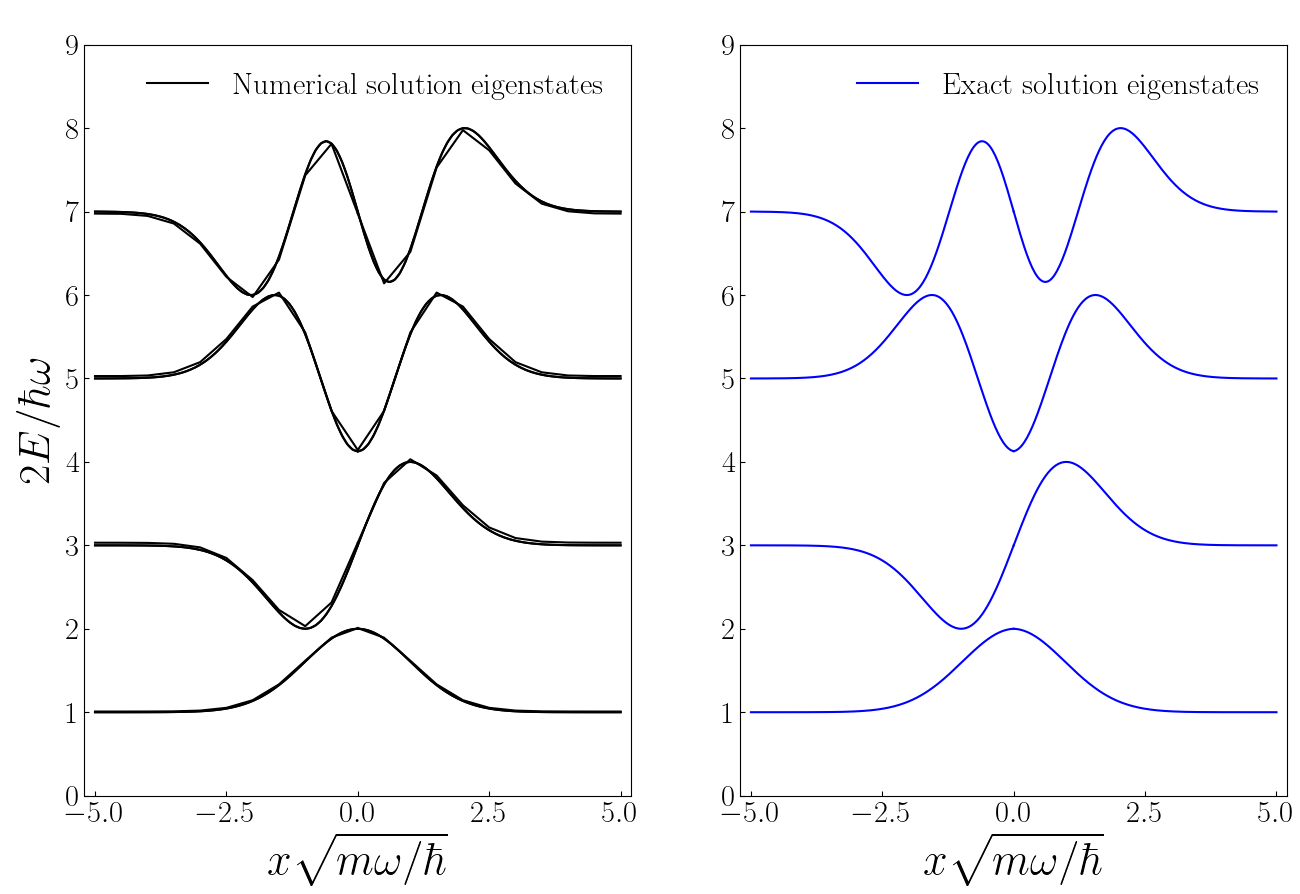
\includegraphics[scale=0.28]{comparison.png}
    \caption{Comparison between exact solution and numerical solution using the inverse power method for the quantum harmonic oscillator. The step sizes used in the numerical solution above were $h=0.025$, $0.1$ and $0.5$.}
    \label{2apr2208}
\end{figure}
The inverse power iteration worked quite well on the quantum harmonic oscillator. A run over the first 50 eigenstates gave a maximum deviation of 0.0013 (in reduced units) from the true energy value. The first four eigenstates are plotted in figure \ref{2apr2208} along with the exact solutions. The numerical solution seems to agree well with the exact solution even for quite large step sizes. 



\begin{figure}
    \centering
    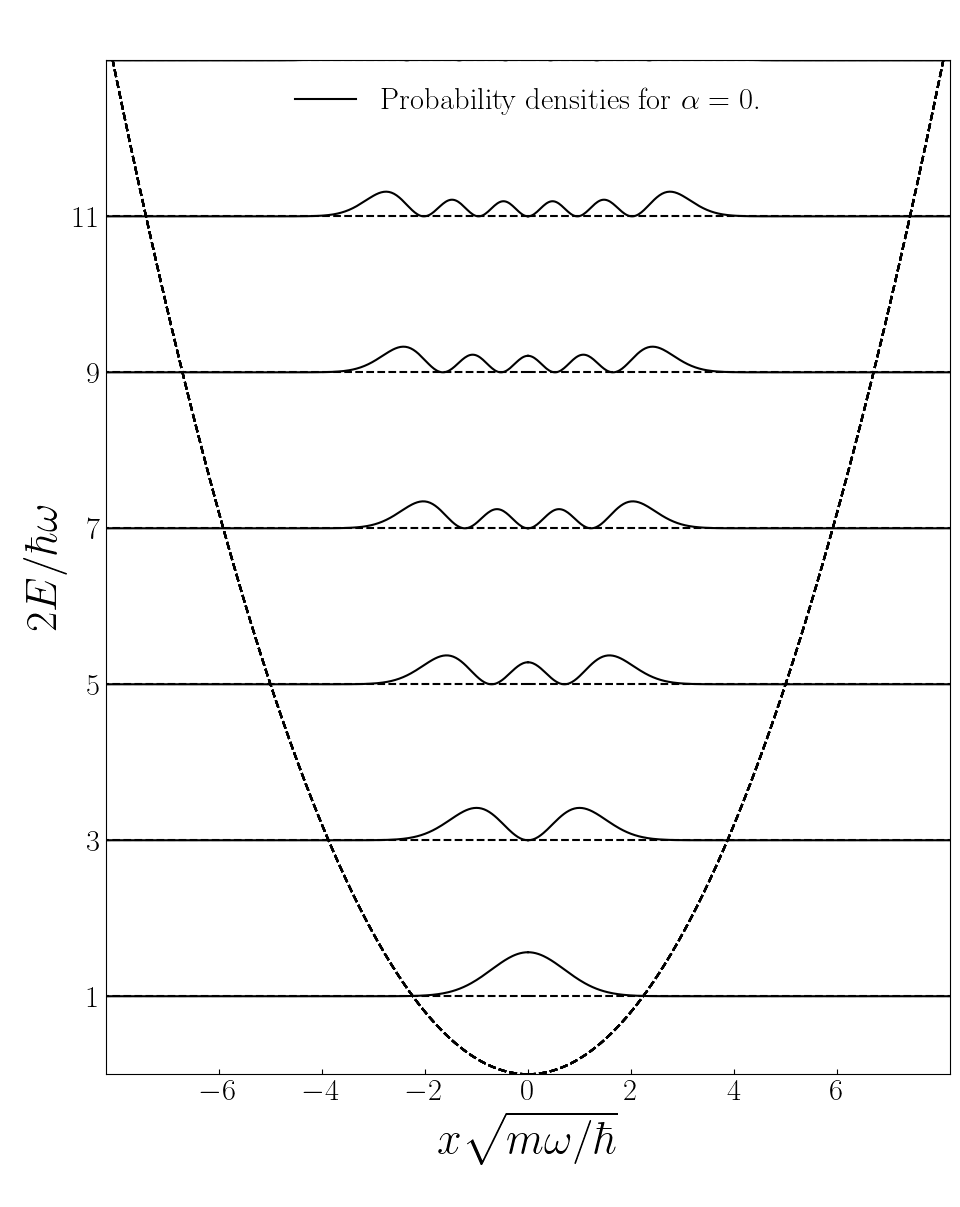
\includegraphics[scale=0.35]{har_osc_density.png}
\end{figure}
\begin{figure}
    \centering
    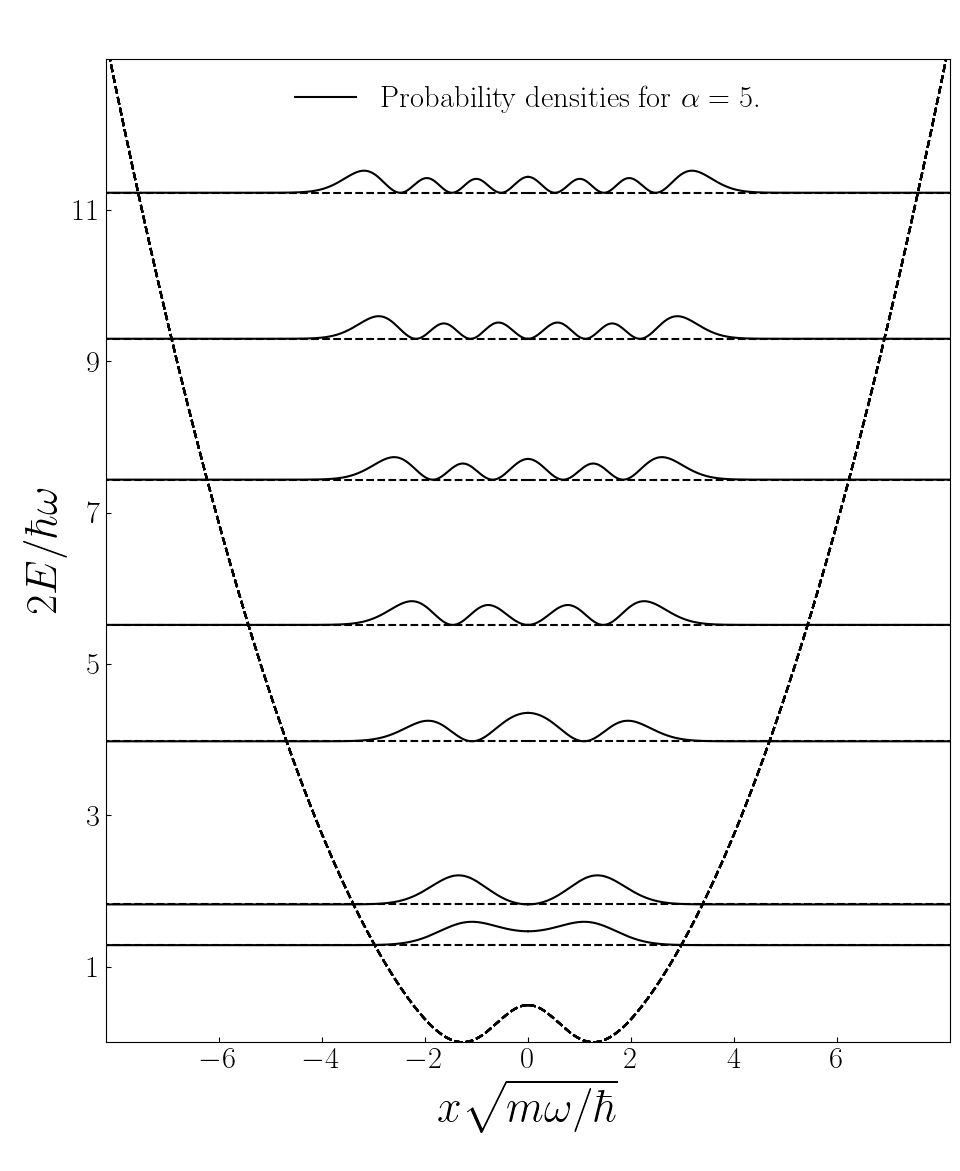
\includegraphics[scale=0.35]{alpha5_density.png}
\end{figure}
\newpage
\blindtext
\begin{figure}
    \centering
    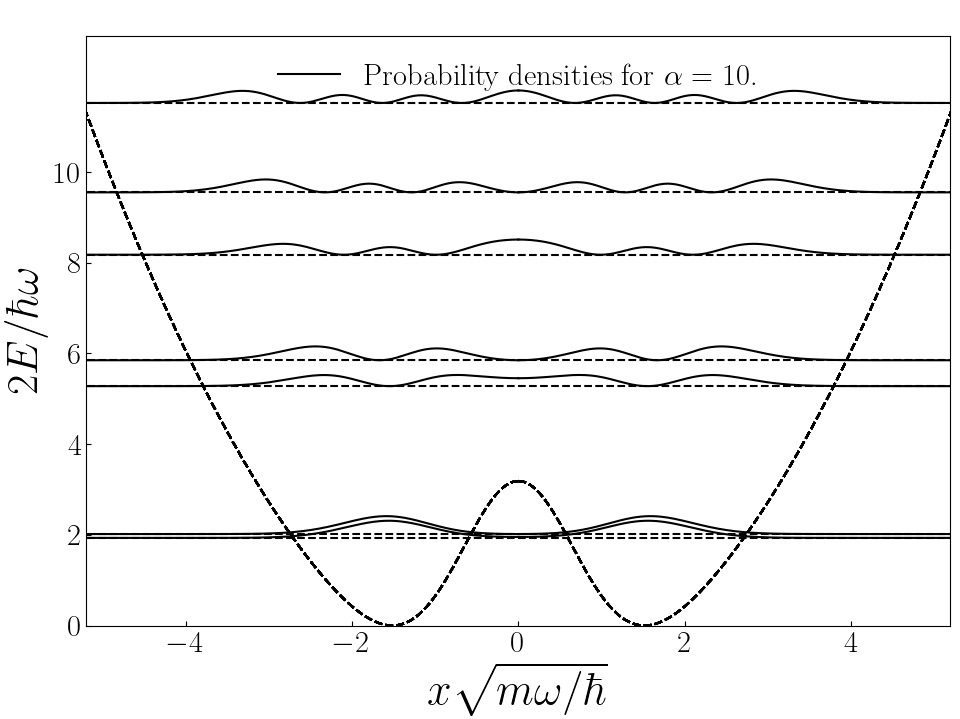
\includegraphics[scale=0.35]{alpha10_density.png}
\end{figure}
\begin{figure}
    \centering
    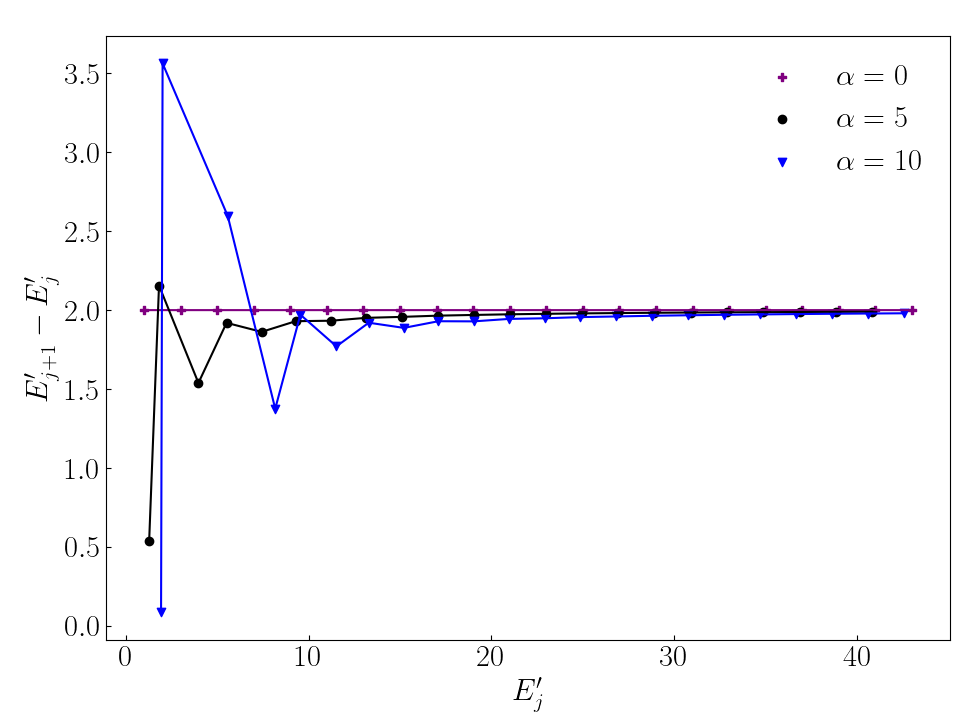
\includegraphics[scale=0.35]{relationship.png}
\end{figure}
%\begin{tabular}{c c c}
%    \centering
%    $E'$ & $|H\mathbf{u}-E'\mathbf{u}|_\text{max}$ & $h$ \\ 
%    \hline\hline \\ 
%    \,\,1.0001 & $7.57\cdot 10^{-8}$ & 0.025 \\ \ 
%    1.0031 & $3.59\cdot 10^{-8}$ & 0.25 \\ \ 
%    1.0083 & $3.77\cdot 10^{-7}$ & 0.5 \\ \ 
%    3.0000 & $3.70\cdot 10^{-6}$ & 0.025 \\ \ 
%    3.0013 & $1.59\cdot 10^{-12}$ & 0.25 \\ \ 
%    3.0316 & $4.97\cdot 10^{-14}$ & 0.5 \\ \ 
%    5.0000 & $1.55\cdot 10^{-6}$ & 0.025 \\ \ 
%    5.0005 & $1.81\cdot 10^{-12}$ & 0.25 \\ \ 
%    5.0288 & $3.41\cdot 10^{-13}$ & 0.5 \\ \ 
%    %7.0070 & $4.01\cdot 10^{-7}$ & 0.025 \\ \ 
%    %7.0070 & $3.69\cdot 10^{-13}$ & 0.25 \\ \ 
%\end{tabular}
\subsection*{Numerical solution to eigenvalue problem}
We wish to solve \eqref{29mar1748} numerically by discretizing the real line and the second derivative of $u$. In order to do so, we introduce the gridpoints $\xi_j$  and the approximations of the function $u$ at these gridpoints, $u_j\approx u(\xi_j)$. Furthermore, we assume that $\xi_j\in[-L,L]$, where $L$ is chosen such that $u(\xi)\approx 0$ for $|\xi|\geq L$. Since the eigenfunctions of an even potential can be taken to be even or odd, we can focus on the interval $[0,L]$ and apply the boundary conditions 
\begin{equation}
    \begin{split}
        &u'(0) = 0 \quad\text{and}\quad u(L) = 0 \quad \text{for even } u, \\ 
        &u(0) = 0 \quad\text{and}\quad u(L) = 0 \quad \text{for odd } u.
    \end{split}
\end{equation} 
The second derivative is approximated up to fourth order:
\begin{equation}
    \begin{split}
        u''(x_j) &\approx \frac{1}{12h^2}\big(-u_{j-2}+16u_{j-1}-30u_j \\ 
        &\hspace{1.7cm}+16u_{j+1}-u_{j+2}\big) 
    \end{split}
\end{equation}

\newpage
\newpage
\subsection*{Appendix: Construction of finite difference matrices}
Here, the following difference formula is chosen:
\begin{equation}
    \begin{split}
        u''(x_j) &= \frac{1}{12h^2}\big(-u(\xi_{j-2})+16u(\xi_{j-1})-30u(\xi_j) \\ 
        &\hspace{1.7cm}+16u(\xi_{j+1})-u(\xi_{j+2})\big) + O(h^4)
    \end{split}
\end{equation}
where $h$ is the step size $h = \xi_{j+1} - \xi_j$ which is assumed to be constant.
For $H_\text{odd}$, one can use a skewed difference formula for the second derivative:
\begin{equation}
    \begin{split}
    u''(h) &= \frac{1}{12h^2}\big(10u(0)-15u(h)-4u(2h) \\
    &\hspace{1.2cm} +14u(3h)-6u(4h)+u(5h)\big) + O(h^4)
    \end{split}
\end{equation}
where $u(0) = 0$. 
Special care had to be taken at the boundaries. For the even case, two ghost points, $\xi_{-1}$ and $\xi_{-2}$, were introduced to the left of zero and two fourth order approximations of the first derivative used to  (... words ...) :

\begin{equation}
    \begin{split}
        &u'(0) \approx \frac{1}{12h}\left(u_{-2}-8u_{-1}+8u_1-u_2\right) \\ 
        &u'(0) \approx \frac{1}{12h}\left(-3u_{-1}-10u_0+18u_1-6u_2+u_3\right)
    \end{split}
\end{equation}


\end{large}
\end{document}
